\documentclass{scrbook}
\usepackage{graphicx} % Required for inserting images
\usepackage{tabularx} % Required for fixed width tables
\usepackage{scrlayer-scrpage} % Required for the subtitles
\usepackage{url} % Required for the URLs
\usepackage{hyperref} % Required for the URLs
\usepackage{listings} % Required for the code snippets
\usepackage{mathtools} % Required for the system of equations
\usepackage{enumitem} % Required for list styling

\usepackage{fontspec}
\setmonofont{DejaVu Sans Mono} % Overleaf has this font pre-installed

% Put the caption of the snippets at the bottom
\lstset{
	captionpos=b,
	basicstyle=\ttfamily\small,
	columns=fullflexible,
	keepspaces=true
}


\title{OWL: Web Ontology Language}
\subtitle{Ambient intelligence course (A.Y. 2025/2026)\\Topic taught by Prof. Floriano Scioscia}
\author{Gabriele Colapinto}
\date{\today}

\begin{document}
	
	\maketitle
	\thispagestyle{empty}
	
	{\Large\textbf{License}} \\
	{Notes from Ambient intelligence (A.Y. 2025/2026) by Gabriele Colapinto. 
		Course taught by professors Michele Ruta, Floriano Scioscia, Arnaldo Tomasino, Davide Loconte — 
		Licensed under CC BY-NC 4.0.\\
		\url{https://creativecommons.org/licenses/by-nc/4.0/}}
	
	\vspace*{\fill}
	\rule{\textwidth}{0.2pt}
	\small{© 2025 Gabriele Colapinto \\
		Released under the \href{https://creativecommons.org/licenses/by-nc/4.0/}{Creative Commons Attribution–NonCommercial 4.0 International License}}
	
	\clearpage
	
	\tableofcontents
	
	\chapter{The Web Ontology Language and OWL 2 Representations}
	
	\section{Purpose of OWL}
	
	The Web Ontology Language, usually abbreviated as OWL, is a Semantic Web language for representing structured knowledge about entities, classes of entities, and relations among them. Its role is not merely to encode data, but to provide a formal vocabulary and a logic-based semantics that make knowledge machine-processable.\\
	
	An OWL document is an ontology: a formal specification of the concepts, individuals, and relationships that describe a domain. Once knowledge is represented in OWL, automated tools can exploit its logical structure to verify whether the ontology is consistent and to derive implicit knowledge that is not explicitly asserted. This distinguishes OWL from data interchange formats that only preserve asserted facts without assigning them a deductive interpretation.\\
	
	OWL is part of the W3C Semantic Web technology stack and is designed for publication and exchange on the World Wide Web. The first version of OWL was standardized in 2004. The current version, OWL 2, was standardized in 2012 and extends the original language with additional modelling constructs, profiles, syntaxes, and clarified semantics.
	
	\section{The OWL 2 Specification Landscape}
	
	OWL 2 is defined by a family of documents with different roles. Some documents are aimed at ontology users and engineers, whereas others provide the normative technical basis for implementers of tools and reasoners. The specification landscape can be organized as follows.
	
	\subsection{User-Oriented Documents}
	
	The \textbf{Document Overview} provides a compact entry point to OWL 2 and explains its relationship with OWL 1. It is the natural starting point because it connects the different specification documents and summarizes the main organization of the standard.\\
	
	The \textbf{OWL 2 Primer} gives an approachable introduction to the language. It is particularly useful when the goal is to understand the modelling constructs before studying their formal definition.\\
	
	The \textbf{OWL 2 New Features and Rationale} document explains the main additions introduced by OWL 2 and motivates their inclusion in the language.\\
	
	The \textbf{OWL 2 Quick Reference Guide} provides a concise guide to the constructs of OWL 2 and highlights the differences with respect to OWL 1.
	
	\subsection{Core Specification Documents}
	
	The \textbf{Structural Specification and Functional-Style Syntax} defines the abstract structure of OWL 2 ontologies and the functional-style syntax used to write them in a form close to the formal data model. It also defines OWL 2 DL (Description Language) ontologies through global restrictions on the structure of OWL 2 ontologies.\\
	
	The \textbf{Mapping to RDF Graphs} specifies how OWL 2 constructs are represented as RDF graphs. This mapping is central to interoperability in the Semantic Web because RDF graphs are the primary exchange model for linked data.\\
	
	The \textbf{Direct Semantics} defines the meaning of OWL 2 ontologies through a model-theoretic semantics. This semantics is closely related to description logics and is the reference point for OWL 2 DL reasoning.\\
	
	The \textbf{RDF-Based Semantics} defines the meaning of OWL 2 ontologies as an extension of RDF semantics. This semantic view is suitable for RDF graphs and for tools that operate directly over graph-based data.\\
	
	The \textbf{Conformance} document defines requirements for OWL 2 tools and provides test cases that support the assessment of conformance.
	
	\subsection{Profiles and Companion Syntaxes}
	
	\begin{figure}
		\centering
		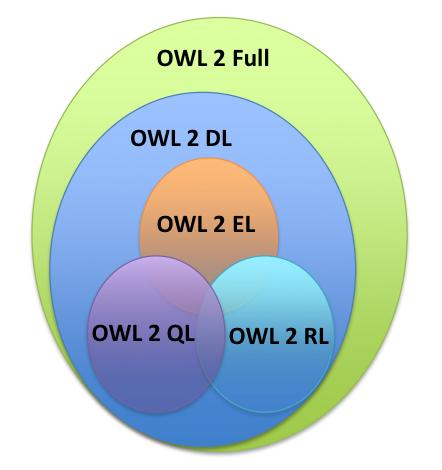
\includegraphics[width=0.5\linewidth]{Images/OWL_2_classifications.jpg}
		\caption{OWL 2 profiles}
		\label{fig:owl_2_profiles}
	\end{figure}
	
	The \textbf{Profiles} specification defines three OWL 2 sublanguages: OWL 2 EL, OWL 2 QL, and OWL 2 RL (see figure \ref{fig:owl_2_profiles}). These profiles restrict the structure of ontologies in order to obtain important computational advantages in specific application scenarios.\\
	
	The \textbf{XML Serialization} specification defines an XML syntax for exchanging OWL 2 ontologies. It is useful when ontologies must be processed with XML-based tools such as schema-aware editors, XQuery processors, or XPath-based workflows.\\
	
	The \textbf{Manchester Syntax} specification defines a syntax that is less formal than the functional-style syntax but easier to read and write. It is widely used in ontology editing interfaces because it provides a compact textual notation for common modelling patterns.\\
	
	The \textbf{Data Range Extension: Linear Equations} document specifies an optional extension for advanced constraints on data values. It is not part of the core modelling vocabulary required for ordinary ontology development, but it illustrates how OWL 2 can be extended with specialized datatypes and constraints.
	
	\section{Abstract Structure of OWL 2 Ontologies}
	
	\begin{figure}[!h]
		\centering
		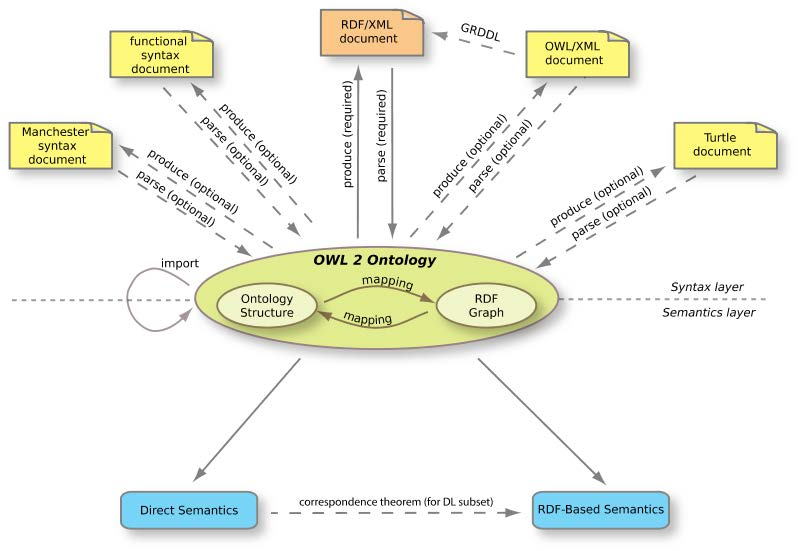
\includegraphics[width=0.5\linewidth]{Images/OWL_2_structure.jpg}
		\caption{OWL 2 abstract structure}
		\label{fig:owl_2_structure}
	\end{figure}
	
	An OWL 2 ontology can be understood at two complementary levels. At the abstract level, it is a structured collection of axioms, declarations, annotations, and import information ("Ontology Structure" in figure \ref{fig:owl_2_structure}). At the exchange level, it can be represented as an RDF graph ("RDF Graph" in figure \ref{fig:owl_2_structure}). The relationship between the abstract ontology structure and RDF graphs is defined by the OWL 2 mapping to RDF graphs.\\
	
	This distinction is important because OWL is not tied to a single concrete syntax. The same ontology can be serialized in several syntactic forms, each optimized for a different purpose. A tool may expose an ontology in a user-friendly syntax, store it in an XML-based representation, and exchange it as RDF triples, without changing the logical content of the ontology.\\
	
	OWL 2 also provides two semantic specifications. The direct semantics assigns meaning to OWL 2 ontologies by interpreting individuals, classes, and properties in a model-theoretic structure. It is the semantics normally associated with OWL 2 DL and with description-logic-based reasoners. The RDF-based semantics instead extends RDF semantics and applies to RDF graphs that may contain OWL vocabulary. The two perspectives support different implementation styles: one focuses on structured OWL axioms, the other on graph-based data.
	
	\section{Concrete Syntaxes}
	
	A concrete syntax determines how an ontology is written, stored, or exchanged. The choice of syntax does not by itself change the ontology's meaning, but it affects readability, tool support, and the ease with which the ontology can be processed.
	
	\subsection{RDF/XML}
	
	\texttt{RDF/XML} is mandatory for OWL 2 tools that claim support for OWL 2 exchange. Its main advantage is interoperability with RDF infrastructure. Since OWL 2 ontologies can be mapped to RDF graphs, RDF/XML provides a standard XML-based serialization of those graphs. Its main drawback is that the syntactic form is often verbose and less readable for humans than syntaxes designed directly for ontology modelling.
	
	\subsection{OWL/XML}
	
	\texttt{OWL/XML} is an XML syntax designed specifically for OWL. It is generally easier to process with XML tools than RDF/XML because the XML structure follows OWL constructs more directly. It is suitable when integration with XML technologies is important and when the ontology is treated primarily as an OWL document rather than as a generic RDF graph.
	
	\subsection{Functional-Style Syntax}
	
	The functional-style syntax is close to the abstract structure of OWL 2. It represents axioms and expressions using constructor names with ordered arguments. This makes the formal organization of the ontology explicit and reduces ambiguity when discussing the language at the specification level.\\
	
	For example, the assertion that \texttt{:Mary} is an instance of \texttt{:Person} is written as follows:
	\begin{lstlisting}
ClassAssertion( :Person :Mary )
	\end{lstlisting}
	
	The functional-style syntax is particularly useful for technical explanations because nested expressions make the structure of complex axioms visible.
	
	\subsection{Manchester Syntax}
	
	Manchester Syntax is designed for readability and for manual ontology editing. It is common in ontology engineering tools because it resembles a controlled textual notation rather than a low-level exchange format. The same assertion about Mary can be written as follows.
	
	\begin{lstlisting}
Individual: Mary
  Types: Person
	\end{lstlisting}
	
	The syntax is less formal as an exchange representation, but it is often more convenient for ontology engineers who need to inspect and modify class descriptions, restrictions, and assertions.
	
	\subsection{Turtle}
	
	Turtle is a compact textual syntax for RDF triples. Since OWL 2 ontologies can be mapped to RDF graphs, Turtle is convenient when the ontology is handled together with RDF data. The assertion that Mary is a person can be represented by the following triple.
	
	\begin{lstlisting}
:Mary rdf:type :Person .
	\end{lstlisting}
	
	Turtle is generally easier to read and write than RDF/XML when the ontology is viewed as a set of RDF triples.
	
	\subsection{Comparing Equivalent Serializations}
	
	The following examples express the same basic assertion in different syntactic forms. In RDF/XML, the class can appear as the XML element and the individual is identified through \texttt{rdf:about}.
	
	\begin{lstlisting}
<Person rdf:about="Mary"/>
	\end{lstlisting}
	
	In OWL/XML, the same assertion is represented with elements corresponding directly to the OWL axiom and its arguments.
	
	\begin{lstlisting}
<ClassAssertion>
  <Class IRI="Person"/>
  <NamedIndividual IRI="Mary"/>
</ClassAssertion>
	\end{lstlisting}
	
	These serializations differ in surface notation, not in intended logical content. The relevant engineering choice is therefore pragmatic: RDF/XML maximizes mandatory exchange support, OWL/XML supports XML-oriented processing, functional-style syntax exposes the formal structure, Manchester Syntax improves human readability, and Turtle provides a concise RDF triple representation.
	
	\section{Consequences for Ontology Engineering}
	
	OWL 2 separates the logical content of an ontology from its concrete representation. This separation allows ontology engineers to choose the syntax that best fits the task while preserving the same underlying axioms. A modelling tool may display axioms in Manchester Syntax, a reasoner may consume a structural representation close to functional-style syntax, and a data integration pipeline may publish the same content as RDF.\\
	
	The coexistence of direct and RDF-based semantics also reflects two complementary uses of OWL. In ontology-centred workflows, OWL axioms are manipulated as structured logical statements and submitted to reasoners that check consistency and derive implicit knowledge. In graph-centred workflows, OWL vocabulary is embedded in RDF data and interpreted through RDF-compatible semantics. Both views are part of the OWL 2 ecosystem, and the appropriate choice depends on the expected reasoning tasks, the expressiveness of the ontology, and the surrounding data infrastructure.
	
	\chapter{OWL 2 Profiles}
	
	\section{Profiles as Lightweight Sublanguages}
	
	OWL 2 profiles are syntactic fragments of OWL 2 designed to preserve useful forms of modelling while improving the computational behaviour of reasoning. A profile restricts the structure of admissible ontologies: not every OWL 2 construct, nor every combination of constructs, is allowed. These restrictions are not merely stylistic. They determine which reasoning algorithms can be applied efficiently and which kinds of ontologies can be handled at practical scale.\\
	
	The need for profiles comes from the tension between expressiveness and computational tractability. Full OWL 2 DL (Description Language) supports a rich combination of constructors, including complex class descriptions, property restrictions, equality, disjointness, cardinalities, inverse properties, and property chains. This expressiveness is valuable when a domain requires precise modelling, but the interaction of these constructs can make reasoning expensive. Profiles address this by selecting coherent subsets of the language that support efficient reasoning for different application scenarios.\\
	
	The three standard profiles are:
	\begin{itemize}
		\item \texttt{OWL 2 EL (Existential Language)}, intended for ontologies with very large numbers of classes and properties;
		\item \texttt{OWL 2 QL (Query Language)}, intended for ontology-based access to very large volumes of instance data;
		\item \texttt{OWL 2 RL (Rule Language)}, intended for scalable rule-based reasoning, especially over RDF-style data.
	\end{itemize}
	
	The choice of a profile depends on the shape of the ontology and on the required reasoning task.
	\begin{itemize}
		\item A taxonomy-rich ontology with many class inclusions and existential dependencies suggests \texttt{OWL 2 EL};
		\item a database-backed knowledge base whose main operation is query answering suggests \texttt{OWL 2 QL};
		\item an application that materializes consequences by rule application suggests \texttt{OWL 2 RL}.
	\end{itemize}
	
	The profiles are not ordered by expressiveness in a simple hierarchy. They overlap, but each profile admits combinations of features that are not available in the others. This is why the profile choice is an engineering decision rather than a matter of selecting the ``largest'' lightweight language.
	
	\section{Computational Motivation}
	
	A reasoner is expected to be sound, and often complete, with respect to the intended semantics of the ontology language. Soundness ensures that every derived conclusion is entailed; completeness ensures that all relevant entailed conclusions of the target kind are derivable. For expressive ontology languages, sound and complete reasoning may require complex algorithms whose worst-case behaviour is high. Profiles reduce this burden by constraining the permitted constructors and their positions inside axioms.\\
	
	The key design principle is that the restrictions should preserve the reasoning tasks needed by the intended application class.
	\begin{itemize}
		\item For \texttt{OWL 2 EL}, the central task is usually classification: computing the subclass hierarchy induced by the ontology.
		
		\item For \texttt{OWL 2 QL}, the central task is query answering over large ABoxes, often delegated to database engines after rewriting the query.
		
		\item For \texttt{OWL 2 RL}, the central task is deriving consequences by a rule engine, typically by applying a finite set of inference rules until saturation.
	\end{itemize}
	
	The practical advantage of profiles is therefore twofold. First, profile-specific reasoners can exploit specialised algorithms that are simpler than general OWL 2 DL reasoning. Second, the restrictions make performance more predictable on large ontologies or datasets. This does not mean that every operation is trivial or that every implementation scales linearly, but it makes the profile suitable for scenarios where unrestricted OWL 2 DL would be unnecessarily costly.
	
	\subsection{Terminological and Assertional Knowledge}
	
	In the Description Logic tradition, an ontology is often conceptually divided into a terminological component and an assertional component. This distinction is useful when discussing OWL reasoning, even though OWL itself presents ontologies as sets of axioms rather than as physically separate boxes.\\
	
	The \textbf{TBox}, or terminological box, contains schema-level knowledge about the domain. It defines the conceptual structure of the ontology through axioms involving classes and properties. Typical TBox axioms include subclass relations, class equivalences, disjointness constraints, property hierarchies, and domain and range restrictions. For example, the statement that every woman is a person, or that \texttt{hasWife} has domain \texttt{Man} and range \texttt{Woman}, belongs to the terminological part of the ontology.\\
	
	The \textbf{ABox}, or assertional box, contains facts about named individuals. It records which individuals belong to which classes and which property relationships hold between individuals or between individuals and data values. For example, assertions stating that \texttt{John} is a \texttt{Person}, that \texttt{John} has wife \texttt{Mary}, or that \texttt{John} has age \texttt{51} are ABox assertions.\\
	
	This distinction is especially important for understanding the OWL 2 profiles. In \texttt{OWL 2 EL}, reasoning is typically oriented toward large terminologies with many classes and properties. In \texttt{OWL 2 QL}, the TBox is used as a schema layer for rewriting queries, while the ABox may contain very large volumes of instance data managed by database systems. In \texttt{OWL 2 RL}, rule-based reasoning often starts from explicit ABox facts and incrementally derives additional assertions using the ontology axioms.
	
	\section{\texttt{OWL 2 EL}}
	
	\subsection{Purpose and Modelling Style}
	
	\texttt{OWL 2 EL} is designed for ontologies with a large number of classes and properties, especially those dominated by class hierarchies and existential relationships. It is based on the \emph{EL} family of description logics, whose characteristic construct is existential restriction. The profile is well suited to domains where the ontology mainly describes categories, parts, processes, and structured dependencies between classes.\\
	
	A typical \texttt{OWL 2 EL} ontology may contain many axioms of the form ``every instance of this class has some relation to an instance of that class''. Such axioms are common in biomedical, chemical, engineering, and product-structure ontologies. The important point is that the ontology may be very large at the schema level, while reasoning remains tractable for the basic reasoning problems targeted by the profile.\\
	
	For example, a domain ontology can state structural dependencies without enumerating individuals:
	\begin{lstlisting}
Class: Cardiomyocyte
  SubClassOf: MuscleCell

Class: HeartWall
  SubClassOf: Tissue and partOf some Heart

Class: Heart
  SubClassOf: Organ

ObjectProperty: partOf
  SubPropertyOf: relatedTo
	\end{lstlisting}
	
	The axiom \texttt{partOf some Heart} expresses an existential condition: each \texttt{HeartWall} is related by \texttt{partOf} to at least one \texttt{Heart}. This kind of modelling is natural for large terminological ontologies because it captures structural regularities without requiring explicit instance data.
	
	\subsection{Reasoning Characteristics}
	
	The main reasoning task in \texttt{OWL 2 EL} is classification. Given a large set of class axioms, the reasoner computes the implicit subclass relationships that follow from them. The profile is designed so that such reasoning can be performed in polynomial time for the relevant basic tasks.\\
	
	Reasoning in \texttt{OWL 2 EL} is commonly implemented by saturation or completion algorithms. These algorithms repeatedly add consequences until no rule can produce new information. In a classification setting, the derived consequences are typically new subclass inclusions. The computation is monotonic: adding derived information does not invalidate earlier derivations, and the process terminates because only finitely many relevant class relationships can be generated from the ontology vocabulary.\\
	
	The benefit of \texttt{OWL 2 EL} is obtained by avoiding constructs whose interaction would destroy the desired complexity properties. In particular, unrestricted negation, unrestricted disjunction, and arbitrary universal restrictions are not part of the core modelling style of the profile. The profile is therefore expressive for positive, structural knowledge, but deliberately limited for modelling alternatives, exclusions, and constraints involving all property successors.
	
	\subsection{Typical Use Cases}
	
	\texttt{OWL 2 EL} is appropriate when:
	\begin{itemize}
		\item the ontology contains many classes and object properties;
		\item the most important task is classification of the schema;
		\item existential dependencies are central to the modelling problem;
		\item the knowledge base is mostly terminological rather than dominated by massive instance data;
		\item efficient incremental maintenance of class hierarchies is important.
	\end{itemize}
	
	It is less appropriate when the application requires expressive negation, complex disjunctions, extensive use of inverse properties, or database-style query answering over very large ABoxes as the primary operation.
	
	\section{\texttt{OWL 2 QL}}
	
	\subsection{Purpose and Modelling Style}
	
	\texttt{OWL 2 QL} is designed for applications with very large volumes of instance data and relatively lightweight ontological structure. The name refers to its orientation toward query answering. The profile is closely related to the \texttt{DL-Lite} family of description logics and is particularly suitable for ontology-based data access.\\
	
	In an ontology-based data access architecture, the ontology provides a conceptual layer over data that may reside in relational databases or other structured repositories. Users formulate queries in terms of ontology classes and properties; the system rewrites these queries into queries over the underlying data. The ontology enriches the schema without requiring all inferred facts to be materialised in advance.\\
	
	A simple example is a university data model in which the ontology abstracts over database-level relations:
	\begin{lstlisting}
Class: Student
  SubClassOf: Person

Class: Course
  SubClassOf: AcademicEntity

ObjectProperty: enrolledIn
  Domain: Student
  Range: Course

ObjectProperty: teaches
  Domain: Professor
  Range: Course
	\end{lstlisting}
	
	A query for all persons can return explicit persons as well as students, because \texttt{Student} is a subclass of \texttt{Person}. The important feature is that this inference can be reflected in the query rewriting, so that a database engine can answer the rewritten query over the explicit data.
	
	\subsection{Query Rewriting}
	
	The characteristic reasoning method for \texttt{OWL 2 QL} is query rewriting. Instead of saturating all facts in the data, the system rewrites an ontology-level query into a set of lower-level queries that already account for the relevant TBox axioms. The rewritten query can then be evaluated by a conventional query engine.\\
	
	For instance, suppose the ontology states that every student is a person. A query for persons can be rewritten to also search for students:
	
	\begin{lstlisting}
Original query:
  Person(x)

Using:
  Student SubClassOf Person

Rewritten query:
  Person(x) OR Student(x)
	\end{lstlisting}
	
	This example is intentionally simple, but it captures the operational idea. The ontology is used to transform the query, and the data layer remains responsible for evaluating the result. This is why \texttt{OWL 2 QL} is well matched to systems where the ABox is large and frequently managed by database technology.\\
	
	The restrictions of \texttt{OWL 2 QL} are motivated by the need to keep rewriting finite and manageable. Some constructs that are harmless for classification-oriented reasoning can make query rewriting explode or fail to terminate in a useful form. In particular, existential restrictions in certain positions must be limited, because they can force arbitrarily long chains of anonymous witnesses that cannot be captured by a fixed finite rewriting independent of the data.
	
	\subsection{Typical Use Cases}
	
	\texttt{OWL 2 QL} is appropriate when:
	\begin{itemize}
		\item the ontology is used as a conceptual schema over large instance datasets;
		\item the primary reasoning task is query answering;
		\item the data is stored in database-like systems;
		\item query evaluation should exploit existing query-processing infrastructure;
		\item the ontology schema is comparatively lightweight.
	\end{itemize}
	
	It is less appropriate for rich structural ontologies that require extensive existential modelling with complex fillers, or for applications where deriving and storing a large materialised closure is the preferred computational model.
	
	\section{\texttt{OWL 2 RL}}
	
	\subsection{Purpose and Modelling Style}
	
	\texttt{OWL 2 RL} is designed for scalable reasoning by rule-based engines. It aims to preserve a useful amount of OWL expressiveness while ensuring that reasoning can be implemented through rules applied to explicit facts. The name reflects this rule-language orientation.\\
	
	The profile is especially natural when ontologies are represented as RDF graphs and processed by systems that support forward chaining, backward chaining, or configurable rule sets. Rather than relying on highly specialised description logic procedures, an \texttt{OWL 2 RL} reasoner can apply inference rules that resemble database rules or logic-programming rules.\\
	
	A typical rule-oriented fragment may express property hierarchies, domains, ranges, class inclusions, and selected property characteristics:
	
	\begin{lstlisting}
ObjectProperty: hasMother
  SubPropertyOf: hasParent

ObjectProperty: hasParent
  Domain: Person
  Range: Person

Class: Parent
  EquivalentTo: Person and hasChild some Person
	\end{lstlisting}
	
	The first axiom supports a direct rule-like inference: whenever \texttt{hasMother(x,y)} holds, \texttt{hasParent(x,y)} can be derived. Domain and range axioms similarly derive class membership from property assertions.
	
	\subsection{Rule-Based Saturation}
	
	Reasoning in \texttt{OWL 2 RL} is commonly performed by saturation. The reasoner starts from the explicit graph or ABox and repeatedly applies rules that add entailed facts. Once no new fact can be derived, the saturated dataset can be queried like an expanded database.\\
	
	The following schematic rules illustrate the idea:
	\begin{lstlisting}
IF hasMother(x, y)
THEN hasParent(x, y)

IF hasParent(x, y)
THEN Person(x)

IF hasParent(x, y)
THEN Person(y)
	\end{lstlisting}
	
	These rules correspond to a subproperty axiom, a domain axiom, and a range axiom. In a real \texttt{OWL 2 RL} implementation, the rule set is systematic and covers the supported constructs of the profile. The advantage is that inference can be integrated into rule engines, RDF stores, and data-processing pipelines.\\
	
	\texttt{OWL 2 RL} is often a good compromise when the application needs more expressive modelling than a purely database-oriented profile but still requires scalable reasoning over large datasets. Its limitations are tied to the requirement that reasoning remain rule-friendly. Constructs that would require creating unbounded anonymous structures or solving highly non-local constraints are restricted.
	
	\subsection{Typical Use Cases}
	
	\texttt{OWL 2 RL} is appropriate when:
	\begin{itemize}
		\item the knowledge base contains many explicit facts;
		\item consequences should be materialised or derived by rules;
		\item RDF graph processing is central to the system architecture;
		\item the application benefits from integration with rule engines;
		\item scalability is required without reducing the ontology to a purely query-rewriting setting.
	\end{itemize}
	
	It is less appropriate when the ontology is primarily a very large class hierarchy requiring highly optimised classification, or when the target architecture is relational query rewriting rather than rule-based inference.
	
	\section{Comparison of the Profiles}
	
	\subsection{Different Optimisation Targets}
	
	The profiles differ primarily in what they optimise.\\
	
	\texttt{OWL 2 EL} optimises terminological reasoning over large class and property vocabularies. It is strongest when the ontology describes many categories and positive structural dependencies. Its reasoning methods are especially suited to computing implicit subclass relationships.\\
	
	\texttt{OWL 2 QL} optimises query answering over large ABoxes. It assumes that the main computational cost lies in accessing the instance data and that the ontology can be used to rewrite queries. Its modelling language is intentionally limited so that ontology-mediated queries can be translated into database-style queries.\\
	
	\texttt{OWL 2 RL} optimises rule-based derivation. It represents a balance between expressiveness and scalable forward inference, making it useful for RDF stores and applications where deriving a materialised closure is convenient.
	
	\subsection{Expressiveness Trade-Offs}
	
	No profile is simply a subset of another in the modelling sense relevant to applications. The reason is that each profile restricts different combinations of constructors. A feature may be harmless in one reasoning paradigm and problematic in another. For example, existential restrictions are central in \texttt{OWL 2 EL}, while \texttt{OWL 2 QL} admits them only in controlled forms to preserve query rewriting. Universal restrictions fit naturally into parts of the rule-based treatment of \texttt{OWL 2 RL}, but they are not the core modelling mechanism of \texttt{OWL 2 EL}.\\
	
	The following table summarises the practical distinction.
	
	\begin{center}
		\begin{tabular}{lll}
			\textbf{Profile} & \textbf{Main target} & \textbf{Typical reasoning style} \\
			\texttt{OWL 2 EL} & Large class/property ontologies & Classification by saturation \\
			\texttt{OWL 2 QL} & Large instance datasets & Query rewriting \\
			\texttt{OWL 2 RL} & Scalable rule-based inference & Rule materialisation/saturation \\
		\end{tabular}
	\end{center}
	
	This comparison should be read as an implementation-oriented guideline, not as a formal definition of the profiles. A concrete ontology must still be checked against the syntactic constraints of the selected profile.
	
	\section{Guidelines for Profile Selection}
	
	A suitable profile can often be identified by examining the dominant structure of the ontology and the main reasoning workload.\\
	
	Choose \texttt{OWL 2 EL} when the ontology is large at the schema level and classification is the main task. This is the case for ontologies that model domains through many classes, subclass axioms, property hierarchies, and existential dependencies. The expected benefit is efficient computation of implicit class relationships.\\
	
	Choose \texttt{OWL 2 QL} when the ontology provides a conceptual layer over large instance data and the main task is answering user queries. This is the typical setting of ontology-based data access, where query rewriting allows database systems to perform the expensive data access operations.\\
	
	Choose \texttt{OWL 2 RL} when the system architecture is based on rules or RDF graph processing and it is useful to materialise inferred facts. The expected benefit is scalable inference without abandoning a significant subset of OWL modelling constructs.\\
	
	Profile selection is not only a modelling decision but also a deployment decision. An ontology that is elegant from a knowledge-engineering perspective may be unsuitable for a target reasoner if it falls outside the intended profile. Conversely, accepting a profile restriction can make an ontology easier to deploy, maintain, and reason over at scale.\\
	
	The practical workflow is therefore:
	\begin{enumerate}
		\item identify the main reasoning task: classification, query answering, or rule-based materialisation;
		\item examine whether the ontology is dominated by schema axioms or instance data;
		\item select the profile whose restrictions match that workload;
		\item validate the ontology with tools that report profile violations;
		\item revise modelling choices that introduce constructs outside the selected profile.
	\end{enumerate}
	
	The central lesson is that profiles are not weakened versions of OWL chosen only for convenience. They are carefully designed fragments whose restrictions encode assumptions about reasoning. Using the right profile makes those assumptions explicit and allows ontology-based applications to scale without giving up formal semantics.
	
	\chapter{OWL 2 Basic Notions and Basic Axioms}
	
	\section{Axioms, Entities, and Expressions}
	
	An OWL ontology is a finite set of axioms. An axiom is a formal statement that contributes to the meaning of the ontology: it can assert that an individual belongs to a class, that one class is included in another, that two classes are disjoint, that two names denote the same individual, or that a property has a specified domain and range. The logical consequences of an ontology are obtained from the interaction of all its axioms, not from each axiom in isolation.\\
	
	The atomic symbols occurring in axioms are called entities. At the modelling level, OWL distinguishes three central kinds of entities:
	\begin{itemize}
		\item \textbf{individuals}, which denote objects of the domain;
		\item \textbf{properties}, which denote binary relations or annotation links;
		\item \textbf{classes}, which denote categories or sets of objects.		
	\end{itemize}
	
	For example, an \emph{individual} such as \texttt{:John} may belong to the \emph{class} \texttt{:Person}, and the \emph{property} \texttt{rdf:type} relates an individual to a class by expressing class membership. In RDF-oriented notation, this assertion can be written as:
	\begin{lstlisting}
:John rdf:type :Person .
	\end{lstlisting}
	
	OWL properties are further divided according to the kinds of values they connect:
	\begin{itemize}
		\item \textbf{Object properties} relate individuals to individuals;
		\item \textbf{Datatype properties} relate individuals to literal values;
		\item \textbf{Annotation properties} attach metadata or auxiliary information to ontological objects and normally do not affect the logical classification of domain individuals.
	\end{itemize}
	
	The following examples illustrate the three cases:
	\begin{lstlisting}
\\ Object property: Individual -> Individual
:John :married :Mary .

\\ Datatype property: Individual -> Literal value
:John :hasAge 35 .

\\ Annotation property: Individual -> Auxiliary information
:John rdfs:seeAlso myOwl:John-Doe .
	\end{lstlisting}
	
	The property \texttt{:married} is an object property because both its subject and its object are individuals. The property \texttt{:hasAge} is a datatype property because its value is a literal. The property \texttt{rdfs:seeAlso} is an annotation property because it records additional descriptive information rather than a domain relation used for classification.\\
	
	Expressions are structured descriptions built from entities by means of OWL constructors. A class name such as \texttt{:Person} is an atomic class expression; more complex expressions can be formed by combining classes and properties. For example, the class of male professors can be described as the intersection of \texttt{:Man} and \texttt{:Professor}. In a readable notation, this can be expressed as:
	\begin{lstlisting}
Class: MenProfessor
  EquivalentTo: Man and Professor
	\end{lstlisting}
	
	An expression is not necessarily an axiom by itself. It becomes part of the ontology when it is used inside an axiom, such as a class equivalence, a subclass relation, an assertion about an individual, or a restriction on a property.
	
	\section{Class Axioms}
	
	Class axioms describe relationships among classes. They are the basis for building taxonomies, defining synonyms, and declaring incompatibilities between categories.
	
	\subsection{Subclass Relations}
	
	A subclass axiom states that every instance of one class is also an instance of another class. The axiom:
	\begin{lstlisting}
Class: Woman
  SubClassOf: Person
	\end{lstlisting}
	means that every individual classified as \texttt{Woman} is necessarily classified as \texttt{Person}. The axiom does not state that every person is a woman; it introduces a one-way inclusion. In description-logic notation, the same relation is written as \texttt{Woman} $\subseteq$ \texttt{Person}.\\
	
	Subclass axioms support ontology classification. When several subclass axioms are combined, a reasoner can compute indirect inclusions. For instance, if \texttt{Woman} is a subclass of \texttt{Person}, and \texttt{Person} is a subclass of \texttt{Agent}, then every \texttt{Woman} is also an \texttt{Agent}. This inferred inclusion need not be explicitly written.
	
	\subsection{Class Equivalence}
	
	A class equivalence axiom states that two class descriptions have exactly the same instances. The axiom:
	\begin{lstlisting}
Class: Person
  EquivalentTo: Human
	\end{lstlisting}
	is stronger than a single subclass assertion. It is logically equivalent to two inclusions: every \texttt{Person} is a \texttt{Human}, and every \texttt{Human} is a \texttt{Person}. Equivalence is therefore appropriate only when the two classes are intended to denote the same extension.\\
	
	Equivalence is frequently used to introduce a convenient name for a complex class expression. In that case, the named class becomes a reusable abbreviation whose meaning is fixed by the expression. The definition is not merely documentation: it participates in reasoning and can be used to classify individuals and derive additional subclass relations.
	
	\subsection{Class Disjointness}
	
	A disjointness axiom states that classes cannot share instances. The axiom:
	\begin{lstlisting}
DisjointClasses: Woman, Man
	\end{lstlisting}
	means that no individual can be both a \texttt{Woman} and a \texttt{Man}. If an ontology also entails that the same individual belongs to both classes, the ontology becomes inconsistent unless the conflict can be avoided by another interpretation.\\
	
	Disjointness axioms are important for detecting modelling errors. They do not create a complete partition unless coverage is also specified. Declaring \texttt{Woman} and \texttt{Man} disjoint says that their intersection is empty; it does not say that every \texttt{Person} must belong to one of them.
	
	\section{Property Axioms}
	
	Property axioms describe relationships among properties and constrain the types of their subjects and objects. In OWL, these constraints are logical axioms. They are not merely validation declarations.
	
	\subsection{Property Hierarchies}
	
	A property hierarchy axiom states that one property is more specific than another. The axiom:
	\begin{lstlisting}
ObjectProperty: hasWife
  SubPropertyOf: hasSpouse
	\end{lstlisting}
	means that whenever an individual is related to another by \texttt{hasWife}, the same pair is also related by \texttt{hasSpouse}. Thus, from:
	\begin{lstlisting}
Individual: John
  Facts: hasWife Mary
	\end{lstlisting}
	a reasoner can infer:
	\begin{lstlisting}
Individual: John
  Facts: hasSpouse Mary
	\end{lstlisting}
	
	Property hierarchies are useful when an ontology distinguishes specialised relations while still supporting queries or axioms written over more general relations. A query for spouses can retrieve pairs connected through \texttt{hasWife} because the specialised relation is included in the general one.
	
	\subsection{Object Property Assertions}
	
	An object property assertion states that two individuals are connected by an object property. The assertion:
	\begin{lstlisting}
Individual: John
  Facts: hasWife Mary
	\end{lstlisting}
	states that the individual \texttt{John} is related to the individual \texttt{Mary} through the property \texttt{hasWife}. Object property assertions are part of the assertional component of an ontology, but they can interact with class and property axioms. For example, if \texttt{hasWife} has a domain and a range, the assertion above can imply class membership for both individuals.
	
	\subsection{Negative Object Property Assertions}
	
	A negative object property assertion states that a specific property relation between two individuals does not hold. The axiom:
	\begin{lstlisting}
Individual: Bill
  Facts: not hasWife Mary
	\end{lstlisting}
	does not mean that all wives of \texttt{Bill} are known and that \texttt{Mary} is absent from a closed list. It states only the specific negative fact that the pair \texttt{(Bill, Mary)} is not in the extension of \texttt{hasWife}. If the ontology also entails the positive assertion \texttt{hasWife(Bill, Mary)}, the ontology becomes inconsistent.\\
	
	This distinction is essential because OWL adopts an open-world semantics. Lack of an asserted property value is not evidence that the value is false. Negative assertions must be stated explicitly when the falsity of a specific relation is part of the domain knowledge.
	
	\subsection{Domain and Range of Object Properties}
	
	A domain axiom specifies the class of subjects of a property, and a range axiom specifies the class of objects. For the property \texttt{hasWife}, one may write:
	\begin{lstlisting}
ObjectProperty: hasWife
  Domain: Man
  Range: Woman
	\end{lstlisting}
	
	These axioms support inference. If the ontology contains:
	\begin{lstlisting}
Individual: John
  Facts: hasWife Mary
	\end{lstlisting}
	then the domain axiom entails that \texttt{John} is a \texttt{Man}, and the range axiom entails that \texttt{Mary} is a \texttt{Woman}. Domain and range axioms should therefore be used as semantic commitments, not as database-style checks that merely reject incorrectly typed data.\\
	
	When several domain axioms are given for the same property, they are interpreted conjunctively: using the property entails membership in all declared domain classes. The same applies to multiple range axioms. If the intended meaning is an alternative between several possible classes, an explicit union expression is required.
	
	\section{Individual Equality and Inequality}
	
	OWL does not rely on a unique-name assumption. Different individual names are not automatically interpreted as different objects. Conversely, two different names may denote the same individual unless this is ruled out by inequality assertions or by other axioms.
	
	\subsection{Individual Equality}
	
	An equality axiom states that two names denote the same individual. The axiom:
	\begin{lstlisting}
Individual: James
  SameAs: Jim
	\end{lstlisting}
	means that \texttt{James} and \texttt{Jim} are two names for one object. All facts known about one of the names also apply to the other. If \texttt{James} is asserted to have age \texttt{51}, then the same fact is true of \texttt{Jim}; if \texttt{Jim} is classified as a \texttt{Person}, then \texttt{James} is also classified as a \texttt{Person}.\\
	
	Equality is a powerful modelling construct because it merges information. It should be used only when identity is intended, not merely because two individuals are similar or related.
	
	\subsection{Individual Inequality}
	
	An inequality axiom states that two names denote distinct individuals. The axiom:
	\begin{lstlisting}
Individual: John
  DifferentFrom: Bill
	\end{lstlisting}
	excludes interpretations in which \texttt{John} and \texttt{Bill} are the same object. This can be relevant for cardinality restrictions, keys, and consistency checking, and it is also important when data sources use different identifiers whose distinctness must be made explicit.\\
	
	If an ontology contains both \texttt{SameAs} and \texttt{DifferentFrom} for the same pair of individuals, it is inconsistent. More generally, inconsistencies can arise indirectly when equality propagates facts into combinations forbidden by disjointness, negative property assertions, or datatype constraints.
	
	\section{Datatype Properties}
	
	Datatype properties relate individuals to literal values. A literal combines a lexical form with a datatype, such as an integer, a decimal value, a date, or a string. The assertion:
	\begin{lstlisting}
Individual: John
  Facts: hasAge "51"^^xsd:integer
	\end{lstlisting}
	states that \texttt{John} is related by \texttt{hasAge} to the integer value represented by the literal \texttt{"51"\textasciicircum{}\textasciicircum{}xsd:integer}.\\
	
	Datatype properties are used when the value is not an individual of the domain but a data value. The distinction between object properties and datatype properties is structural: an object property can connect \texttt{John} to \texttt{Mary}; a datatype property can connect \texttt{John} to a literal such as \texttt{51}. The two categories are not interchangeable.
	
	\subsection{Negative Datatype Property Assertions}
	
	A negative datatype property assertion states that a specific individual is not related by a given datatype property to a specific literal value. For example:
	\begin{lstlisting}
Individual: John
  Facts: not hasAge "51"^^xsd:integer
	\end{lstlisting}
	asserts that \texttt{John} does not have \texttt{"51"\textasciicircum{}\textasciicircum{}xsd:integer} as a value of \texttt{hasAge}. As with negative object property assertions, this does not close the property. It does not say that the age is known, nor that \texttt{John} has no age value. It only excludes the specified value.\\
	
	A positive assertion and a negative assertion for the same individual, property, and datatype value are contradictory. Datatype equality can also matter: two lexical forms may denote the same value for a datatype, depending on the datatype semantics.
	
	\subsection{Domain and Range of Datatype Properties}
	
	Domain and range axioms can also be declared for datatype properties:
	\begin{lstlisting}
DataProperty: hasAge
  Domain: Person
  Range: xsd:nonNegativeInteger
	\end{lstlisting}
	
	The domain axiom entails that any subject of \texttt{hasAge} is a \texttt{Person}. The range axiom constrains values of \texttt{hasAge} to the datatype \texttt{xsd:nonNegativeInteger}. Thus, if an individual is related through \texttt{hasAge} to a value that is incompatible with the declared range, the ontology may become inconsistent.\\
	
	The range of a datatype property should be chosen at the level required by the modelling task. For example, \texttt{xsd:nonNegativeInteger} is appropriate for ages if negative values are impossible by definition, whereas a broader datatype such as \texttt{xsd:integer} would fail to capture that constraint.
	
	\section{Annotation Properties}
	
	Annotation properties encode information about ontology entities, axioms, or individuals that is useful for documentation, linkage, provenance, or user interfaces. Examples include labels, comments, version information, and cross-references such as \texttt{rdfs:seeAlso}. An annotation such as:
	\begin{lstlisting}
:John rdfs:seeAlso myOwl:John-Doe .
	\end{lstlisting}
	can connect \texttt{:John} to an external description without asserting an object-level domain relation such as marriage, parenthood, membership, or ownership.\\
	
	Annotation properties should not be used when the relation is intended to participate in domain reasoning. If a property should affect classification, consistency, property hierarchies, or query answering over the domain model, it should be represented as an object property or datatype property as appropriate.
	
	\section{Modelling Consequences of Basic Axioms}
	
	Even the basic axioms introduced in this chapter are enough to produce non-trivial inferences. Consider the following small ontology fragment:
	\begin{lstlisting}
Class: Woman
  SubClassOf: Person

Class: Man
  SubClassOf: Person

DisjointClasses: Woman, Man

ObjectProperty: hasWife
  SubPropertyOf: hasSpouse
  Domain: Man
  Range: Woman

Individual: John
  Facts: hasWife Mary
	\end{lstlisting}
	
	From these axioms a reasoner can infer that \texttt{John} has \texttt{Mary} as spouse, that \texttt{John} is a \texttt{Man}, that \texttt{Mary} is a \texttt{Woman}, and that both are \texttt{Person}s. None of these consequences needs to be asserted separately:
	\begin{lstlisting}
Individual: John
  Types: Man, Person
  Facts: hasSpouse Mary

Individual: Mary
  Types: Woman, Person
	\end{lstlisting}
	
	The same fragment can also detect contradictions. If the ontology additionally asserted that \texttt{John} is a \texttt{Woman}, then \texttt{John} would be both a \texttt{Woman} and a \texttt{Man}, contradicting the disjointness axiom. If it asserted that \texttt{John} does not have \texttt{Mary} as wife, it would contradict the positive \texttt{hasWife} assertion. If it asserted that \texttt{John} and \texttt{Mary} are the same individual, the domain and range inferences would classify the same object as both \texttt{Man} and \texttt{Woman}, again conflicting with disjointness.\\
	
	These examples show why basic axioms should be understood semantically. They are not passive schema annotations. They define constraints and entailments that determine how the ontology behaves under automated reasoning.
	
	\chapter{Advanced OWL 2 Class Expressions and Restrictions}
	
	\section{Purpose of Advanced Class Axioms}
	
	OWL 2 class modelling is not limited to named classes and direct subclass hierarchies. Complex class expressions allow a class to be described through logical combinations of other classes and through constraints on the values of properties. These expressions are used inside axioms such as \texttt{SubClassOf}, \texttt{EquivalentTo}, and individual type assertions.\\
	
	The central modelling distinction is between necessary and necessary-and-sufficient conditions. A \texttt{SubClassOf} axiom states a condition that every instance of the subclass must satisfy. An \texttt{EquivalentTo} axiom states both directions: every instance of the named class satisfies the description, and every individual satisfying the description is an instance of the named class. Equivalence axioms are therefore stronger and support classification of implicit instances.\\
	
	The following examples use Manchester-style notation for readability.
	
	\begin{lstlisting}
Class: Mother
  EquivalentTo: Woman and Parent

Class: Grandfather
  SubClassOf: Man and Parent
	\end{lstlisting}
	
	The first axiom defines \texttt{Mother} exactly as the intersection of \texttt{Woman} and \texttt{Parent}. If an individual is inferred to be both a woman and a parent, it can also be inferred to be a mother. The second axiom only states that every grandfather is both a man and a parent; it does not state that every man who is a parent is necessarily a grandfather.
	
	\section{Boolean Class Constructors}
	
	\subsection{Intersection}
	
	The intersection constructor forms a class whose instances belong to all component classes. It corresponds to logical conjunction and is commonly used to express cumulative requirements.
	
	\begin{lstlisting}
Class: Mother
  EquivalentTo: Woman and Parent
	\end{lstlisting}
	
	An individual belongs to \texttt{Mother} precisely when it belongs to both \texttt{Woman} and \texttt{Parent}. Intersections are often used in definitions because they make explicit which independent criteria jointly characterize a concept.
	
	\subsection{Union}
	
	The union constructor forms a class whose instances belong to at least one of the component classes. It corresponds to logical disjunction.
	
	\begin{lstlisting}
Class: Parent
  EquivalentTo: Mother or Father
	\end{lstlisting}
	
	This axiom states that \texttt{Parent} contains all mothers and all fathers, and that every parent is either a mother or a father. Such an equivalence should be used only when the listed alternatives exhaust the intended cases. If the ontology must allow other kinds of parents, a weaker pair of subclass axioms is more appropriate.
	
	\begin{lstlisting}
Class: Mother
  SubClassOf: Parent

Class: Father
  SubClassOf: Parent
	\end{lstlisting}
	
	Union expressions increase modelling expressivity, but they can also make reasoning more expensive. In lightweight profiles, unrestricted use of disjunction is typically avoided because it introduces branching choices in reasoning procedures.
	
	\subsection{Complement}
	
	The complement constructor forms the class of all individuals that are not members of a given class. It corresponds to logical negation.
	
	\begin{lstlisting}
Class: ChildlessPerson
  EquivalentTo: Person and not Parent
	\end{lstlisting}
	
	This axiom defines a childless person as a person who is not a parent. The expression \texttt{not Parent} is a logical complement, not a test for missing data. Under the open-world assumption, the absence of a known child relationship does not by itself imply that an individual is not a parent. To infer membership in \texttt{ChildlessPerson}, the ontology must contain enough information to entail that the individual cannot be a parent.\\
	
	Complement is also related to disjointness. Declaring two classes disjoint can be understood as stating that their intersection is empty, or equivalently that each class is a subclass of the complement of the other.
	
	\begin{lstlisting}
DisjointClasses: Woman, Man
	\end{lstlisting}
	
	If an individual is asserted or inferred to belong to both disjoint classes, the ontology becomes inconsistent.
	
	\section{Restrictions on Object Properties}
	
	Class expressions can also be defined by constraining the objects reached through a property. Such restrictions describe individuals in terms of their relationships with other individuals.
	
	\subsection{Existential Restrictions}
	
	An existential restriction states that at least one property value satisfying a given class condition exists.
	
	\begin{lstlisting}
Class: Parent
  EquivalentTo: hasChild some Person
	\end{lstlisting}
	
	This axiom defines \texttt{Parent} as the class of individuals related through \texttt{hasChild} to at least one individual that is a \texttt{Person}. If the ontology states that \texttt{John} has a child who is a person, then \texttt{John} can be classified as a parent. Conversely, if \texttt{John} is asserted to be a parent, the reasoner can conclude that some person exists as a child of \texttt{John}, even if that child is not explicitly named.\\
	
	Existential restrictions are useful when membership in a class depends on the existence of a relationship. They are also central in profiles that support efficient reasoning over large class hierarchies, because many domain models require class definitions based on parts, participants, locations, or roles.
	
	\subsection{Universal Restrictions}
	
	A universal restriction states that all values of a property, if present, must belong to a given class.
	
	\begin{lstlisting}
Class: HappyPerson
  EquivalentTo: hasChild only HappyPerson
	\end{lstlisting}
	
	This axiom says that all children of a happy person are happy persons. It does not state that a happy person has at least one child. Universal restrictions constrain existing property fillers; they do not create new ones. If existence is also required, the universal restriction must be combined with an existential restriction.
	
	\begin{lstlisting}
Class: HappyParent
  EquivalentTo: hasChild some Person and hasChild only HappyPerson
	\end{lstlisting}
	
	The first conjunct requires at least one child who is a person. The second conjunct requires every child to be a happy person. Together, they express both existence and value constraint.\\
	
	Universal restrictions are also a compact way to express range-like constraints. For example, saying that every value of \texttt{hasChild} must be a \texttt{Person} constrains the second argument of that property.
	
	\begin{lstlisting}
ObjectProperty: hasChild
  Range: Person
	\end{lstlisting}
	
	A range axiom does not reject the property assertion by default. Instead, if \texttt{John hasChild Mary} is present, the reasoner may infer that \texttt{Mary} is a \texttt{Person}. Inconsistency arises only if other axioms make this inferred type impossible.
	
	\section{Cardinality Restrictions}
	
	Cardinality restrictions constrain the number of property values associated with an individual. They can express upper bounds, lower bounds, or exact numbers of fillers. In OWL 2, cardinality restrictions may be qualified by the class of the counted fillers.
	
	\begin{lstlisting}
Individual: John
  Types: hasChild max 4 Parent

Individual: John
  Types: hasChild min 2 Parent

Individual: John
  Types: hasChild exactly 4 Parent
	\end{lstlisting}
	
	The first assertion states that \texttt{John} has at most four children that are parents. The second states that he has at least two such children. The third combines both constraints and states that the number is exactly four.\\
	
	A qualified cardinality restriction counts only fillers belonging to the specified class. Thus, \texttt{hasChild max 4 Parent} does not limit the total number of children of \texttt{John}; it limits only those children that are parents. An unqualified cardinality restriction can be understood as counting fillers in the universal class \texttt{owl:Thing}.\\
	
	Cardinality constraints interact with equality reasoning. OWL does not assume that different individual names denote different objects. If an ontology states that \texttt{John} has five named children and also states that he has at most four children, a reasoner may infer that at least two of the child names denote the same individual, unless the ontology explicitly asserts them to be different. Therefore, cardinality restrictions often require explicit inequality axioms when the intended model depends on distinct named individuals.
	
	\begin{lstlisting}
Individual: John
  Facts: hasChild Ann, Bob, Carl, Diana, Eva
  Types: hasChild max 4 Person

DifferentIndividuals: Ann, Bob, Carl, Diana, Eva
	\end{lstlisting}
	
	With the inequality assertion, the ontology cannot satisfy both the five distinct children and the maximum cardinality of four, so the combination becomes inconsistent if all five children are persons.
	
	\section{Combining Restrictions in Definitions}
	
	Advanced OWL class descriptions are often built by combining Boolean constructors and property restrictions. This makes it possible to define classes intentionally, by the conditions that characterize their instances.
	
	\begin{lstlisting}
Class: Grandfather
  EquivalentTo: Man and Parent and hasChild some Parent
	\end{lstlisting}
	
	This definition states that a grandfather is a man, is a parent, and has at least one child who is also a parent. Depending on the surrounding ontology, the explicit conjunct \texttt{Parent} may be redundant: if \texttt{Parent} is defined as \texttt{hasChild some Person}, then having a child who is a parent already entails having a child who is a person. Such redundancies are not necessarily errors; they may improve readability, but they can also obscure the minimal logical definition.\\
	
	The choice between \texttt{SubClassOf} and \texttt{EquivalentTo} remains important in combined definitions. A necessary condition supports checking whether known instances comply with a model, whereas an equivalence supports automatic classification of individuals and subclasses that satisfy the definition.
	
	\begin{lstlisting}
Class: Grandfather
  SubClassOf: Man and Parent

Class: Grandfather
  EquivalentTo: Man and hasChild some Parent
	\end{lstlisting}
	
	The first axiom constrains known grandfathers. The second can classify an individual as a grandfather when the ontology entails that he is a man and has a child who is a parent.
	
	\section{Reasoning Consequences of Advanced Axioms}
	
	Advanced axioms increase the amount of implicit knowledge that can be derived from an ontology. They support classification, detection of inconsistent class definitions, inference of missing type information, and propagation of constraints through object properties. At the same time, they require careful modelling because OWL uses open-world semantics and does not adopt the unique name assumption.\\
	
	The open-world assumption means that unknown facts are not false by default. A missing \texttt{hasChild} assertion is not enough to infer that a person is childless, and an incomplete list of children is not enough to satisfy a maximum cardinality constraint. Cardinality, complement, and universal restrictions should therefore be interpreted as logical constraints over all possible models, not as database checks over the currently stored facts.\\
	
	The absence of the unique name assumption means that different names may denote the same individual. This is particularly relevant for maximum cardinality restrictions and for equality-based reasoning. When distinctness matters, it must be stated explicitly using inequality axioms.\\
	
	Finally, expressive constructors have computational consequences. Intersections and existential restrictions are compatible with efficient reasoning in important fragments of OWL. Unrestricted disjunction, negation, and qualified cardinality restrictions are more demanding because they create alternatives, exclusions, and counting constraints. The design of an OWL ontology should therefore balance the precision of the intended conceptual model with the reasoning tasks and scalability requirements of the application.
	
	\chapter{Ontology Management and Reasoning Tasks}
	
	\section{Ontology Identification and Modular Organization}
	
	An OWL ontology is not only a set of logical axioms. It is also a managed artefact intended to be stored, exchanged, reused, and processed by tools. For this reason, an ontology normally has an identifier, a set of namespace prefixes, and possibly a set of imports that connect it to other ontologies. These elements do not replace the logical axioms of the ontology, but they determine how the ontology is named, how its terms are abbreviated, and how external knowledge is made available during processing.\\
	
	The ontology identifier is usually an IRI. It gives a stable name to the ontology as a whole and allows tools, applications, and other ontologies to refer to it unambiguously.
	
	\begin{lstlisting}
Ontology: <http://example.com/owl/families>
	\end{lstlisting}
	
	The ontology IRI should be chosen as a persistent identifier rather than as a temporary file location. In many projects, the ontology IRI and the physical URL from which the file is retrieved coincide, but this is not required by the logical model. The important point is that the IRI identifies the ontology as a semantic artefact.
	
	\section{Prefixes and Namespaces}
	
	OWL ontologies typically use IRIs for classes, properties, individuals, and annotations. Since full IRIs are verbose, concrete syntaxes allow prefixes to abbreviate commonly used namespaces. Prefix declarations improve readability and reduce the risk of mistakes when the same namespace is used repeatedly.
	
	\begin{lstlisting}
Prefix: owl:    <http://www.w3.org/2002/07/owl#>
Prefix: poliba: <http://example.org/owl/poliba/>
	\end{lstlisting}
	
	After these declarations, a term such as \texttt{owl:Class} expands to an IRI in the OWL namespace, while a term such as \texttt{poliba:Student} expands to an IRI in the application-specific namespace. Prefixes are syntactic abbreviations: they do not change the logical meaning of the entities they abbreviate. Two prefixed names denote the same entity only if their expanded IRIs are the same.\\
	
	Prefix management is especially important in modular ontologies. A large ontology may reuse standard vocabularies, domain ontologies, and project-specific terms. Clear prefix conventions help distinguish these layers and make the ontology easier to inspect and maintain.
	
	\section{Ontology Imports}
	
	The \texttt{Import} mechanism allows one ontology to include the axioms of another ontology. Importing is stronger than merely referring to an external IRI. When an ontology imports another ontology, reasoning over the importing ontology is performed with the imported axioms available as part of the logical context.
	
	\begin{lstlisting}
Import: <http://example.org/owl/poliba.owl>
	\end{lstlisting}
	
	Imports support modularization. A domain ontology can be separated from upper-level vocabulary, datatype conventions, or application-specific extensions. For example, a family ontology may import a more general ontology of persons, relationships, and demographic attributes. The family ontology can then define specialized concepts while relying on the imported ontology for shared background axioms.\\
	
	Imports must be used carefully. Adding an imported ontology may introduce new subclass relations, property constraints, equivalence axioms, disjointness axioms, or individual assertions. These imported axioms can change classification results, make previously satisfiable classes unsatisfiable, or make the whole ontology inconsistent. Therefore, import closure---the ontology together with all ontologies recursively imported by it---is the effective unit considered by a reasoner.
	
	\section{Editing and Reasoning Tools}
	
	Ontology engineering is normally supported by editing environments that combine syntax management, visualization, validation, and reasoning services. A widely used example is \texttt{Protege}, a free open-source ontology editing framework developed at Stanford University. Such tools allow ontology engineers to create classes, properties, individuals, annotations, restrictions, and imports without directly editing every axiom in a textual syntax.\\
	
	Reasoners are separate components that compute logical consequences of an ontology. They are often integrated into ontology editors, but conceptually they perform a distinct task: given an ontology and a semantics, they determine which axioms follow from the asserted axioms. In the OWL DL setting, examples of reasoners include \texttt{FaCT++}, \texttt{HermiT}, \texttt{Pellet}, \texttt{RacerPro}, and \texttt{Tiny-ME}. They differ in implementation techniques, supported features, performance characteristics, and integration targets, but they share the same general purpose of deriving consequences from formal semantics.\\
	
	The choice of a reasoner depends on the ontology language fragment and on the intended reasoning task. A highly expressive OWL 2 DL ontology may require a complete DL reasoner. A profile-conformant ontology may be handled more efficiently by a specialized reasoner for \texttt{OWL 2 EL}, \texttt{OWL 2 QL}, or \texttt{OWL 2 RL}. In practical workflows, reasoning is not a final step performed only after modelling is complete; it is an iterative validation mechanism used throughout ontology development.
	
	\section{Reasoning Within OWL DL}
	
	Reasoning in OWL DL is based on the formal interpretation of classes as sets of individuals and properties as binary relations. An ontology constrains the possible interpretations of its vocabulary. A model of the ontology is an interpretation that satisfies all asserted axioms. An axiom is entailed when it holds in every model of the ontology.\\
	
	This model-theoretic view explains the difference between asserted and inferred knowledge. An asserted axiom is explicitly present in the ontology. An inferred axiom is not necessarily written in the ontology, but it follows from the asserted axioms. For example, if every \texttt{Woman} is a \texttt{Person} and \texttt{Mary} is asserted to be a \texttt{Woman}, then \texttt{Mary} is inferred to be a \texttt{Person}.
	
	\begin{lstlisting}
Class: Woman
  SubClassOf: Person

Individual: Mary
  Types: Woman
	\end{lstlisting}
	
	From these axioms, a reasoner can derive that \texttt{Mary} belongs to \texttt{Person}. The inferred type is not a separate assumption: it is a logical consequence of the class hierarchy and the individual assertion.\\
	
	Reasoning is also affected by the open-world assumption. The absence of an assertion does not imply that the assertion is false. If no child is listed for an individual, it does not follow that the individual is childless. Similarly, if no type is asserted for an individual, this does not mean that the individual has no type. Reasoners compute what is forced by the ontology, not what is absent from the currently stored data.
	
	\section{Local Reasoning Tasks}
	
	\subsection{Satisfiability}
	
	Satisfiability checks whether a class expression can have at least one instance with respect to the ontology. A class expression is unsatisfiable when the ontology forces it to be empty. Unsatisfiable classes usually indicate contradictory modelling constraints.
	
	\begin{lstlisting}
Class: Woman
  DisjointWith: Man

Class: ImpossiblePerson
  EquivalentTo: Woman and Man
	\end{lstlisting}
	
	Since \texttt{Woman} and \texttt{Man} are disjoint, the intersection \texttt{Woman and Man} cannot have instances. Therefore, \texttt{ImpossiblePerson} is unsatisfiable. This does not automatically make the whole ontology inconsistent: the ontology may still have models as long as no individual is forced to instantiate the unsatisfiable class.\\
	
	Satisfiability is central to ontology validation because it detects modelling errors that may not be visible from isolated axioms. A contradiction often emerges only from the combination of equivalence definitions, disjointness, domains, ranges, and property restrictions.
	
	\subsection{Subsumption}
	
	Subsumption checks whether one class expression is more specific than another with respect to the ontology. If a class expression \texttt{A} is subsumed by a class expression \texttt{B}, then every instance of \texttt{A} is necessarily an instance of \texttt{B}.
	
	\begin{lstlisting}
Class: Mother
  EquivalentTo: Woman and Parent

Class: Parent
  SubClassOf: Person
	\end{lstlisting}
	
	From this ontology, a reasoner can infer that \texttt{Mother} is subsumed by \texttt{Person}, because every mother is a parent and every parent is a person. The inferred subsumption does not need to be asserted directly. Subsumption therefore supports the construction and maintenance of class hierarchies.\\
	
	Subsumption is not limited to named classes. It can also be evaluated between complex class expressions. For example, a class expression requiring a child of type \texttt{Person} may be compared with a broader expression requiring some child of type \texttt{owl:Thing}. Such comparisons are useful when checking whether definitions are redundant, overly general, or more specific than intended.
	
	\subsection{Instance Checking}
	
	Instance checking determines whether a given individual belongs to a given class expression with respect to the ontology. It is the individual-level counterpart of subsumption.
	
	\begin{lstlisting}
Class: Parent
  EquivalentTo: hasChild some Person

Individual: John
  Facts: hasChild Mary

Individual: Mary
  Types: Person
	\end{lstlisting}
	
	The ontology entails that \texttt{John} is an instance of \texttt{Parent}, because he has at least one child who is a person. This conclusion is obtained even if the type assertion \texttt{Parent(John)} is not explicitly present.\\
	
	Instance checking is often used to validate expected classifications of individuals. If a known individual is not inferred to belong to an expected class, the ontology may be missing relevant assertions or definitions. Conversely, an unexpected inferred type may reveal that a definition is too broad or that a domain or range axiom is producing unintended classifications.
	
	\subsection{Instance Retrieval}
	
	Instance retrieval generalizes instance checking. Given a class expression, the task is to retrieve all individuals in the ontology that are entailed to belong to that expression.
	
	\begin{lstlisting}
Class: Parent
  EquivalentTo: hasChild some Person
	\end{lstlisting}
	
	For the class \texttt{Parent}, retrieval returns all named individuals that the ontology entails to have at least one \texttt{hasChild} relation to a person. The result may include individuals whose parenthood is asserted directly and individuals whose parenthood is inferred from property assertions and class definitions.\\
	
	Instance retrieval should not be confused with database selection under a closed-world assumption. A reasoner returns individuals whose membership is logically entailed. It does not return individuals merely because they are plausible candidates, and it does not exclude individuals simply because some facts are missing.
	
	\subsection{Query Answering}
	
	Query answering computes the answers to a query with respect to an ontology. The query is usually expressed in a query language such as \texttt{SPARQL}. Compared with simple instance retrieval, query answering can involve several variables, property paths, joins, filters, and graph patterns.\\
	
	A query may ask for all persons and their children:
	
	\begin{lstlisting}
SELECT ?x ?y
WHERE {
  ?x :hasChild ?y .
  ?y rdf:type :Person .
}
	\end{lstlisting}
	
	When query answering is ontology-aware, answers are computed not only from explicitly stored triples but also from relevant entailments. For example, if \texttt{:Mary} is known to be a \texttt{:Woman} and every woman is a person, then an ontology-aware query engine may use the inferred type \texttt{:Person} when answering the query.\\
	
	The computational behaviour of query answering depends strongly on the chosen OWL fragment. \texttt{OWL 2 QL} is designed precisely for settings in which large amounts of instance data are queried through a relatively lightweight ontology. In such systems, reasoning can often be reduced to query rewriting: the ontology is compiled into an expanded query that can be evaluated by a conventional database engine.
	
	\section{Global Ontology Reasoning Tasks}
	
	\subsection{Ontology Coherence}
	
	Ontology coherence checks whether all named classes in the ontology are satisfiable. An ontology is incoherent if at least one named class cannot have instances. Incoherence is weaker than full inconsistency: useful inferences may still be drawn from coherent parts of an incoherent ontology.
	
	\begin{lstlisting}
Class: Woman
  DisjointWith: Man

Class: ImpossiblePerson
  EquivalentTo: Woman and Man
	\end{lstlisting}
	
	This ontology is incoherent because \texttt{ImpossiblePerson} is unsatisfiable. However, if no individual is asserted or inferred to be an \texttt{ImpossiblePerson}, the ontology may still be consistent. Coherence checking is therefore a diagnostic task aimed at the quality of the conceptual schema.\\
	
	In ontology engineering, incoherent classes often arise from excessive equivalence axioms, incompatible superclass constraints, disjointness axioms, or unintended domain and range consequences. Detecting them early prevents errors from propagating into classification and retrieval tasks.
	
	\subsection{Ontology Consistency}
	
	Ontology consistency determines whether the ontology has at least one model. If an ontology is inconsistent, its axioms cannot be satisfied simultaneously. Under classical semantics, an inconsistent ontology entails every statement, so no useful distinction between true and false consequences remains.
	
	\begin{lstlisting}
Class: Woman
  DisjointWith: Man

Individual: Alex
  Types: Woman, Man
	\end{lstlisting}
	
	The ontology is inconsistent because \texttt{Alex} is forced to be an instance of two disjoint classes. Unlike mere incoherence, this contradiction occurs at the level of the ontology as a whole. Once inconsistency is present, classification and retrieval results cannot be trusted as meaningful logical consequences.\\
	
	Consistency checking is normally the first reasoning task performed during validation. There is little value in inspecting a computed class hierarchy or query result if the ontology is inconsistent. After consistency is restored, coherence and classification can be used to diagnose more localized modelling problems.
	
	\subsection{Ontology Classification}
	
	Ontology classification computes the concept taxonomy induced by the subsumption relation. It is logically equivalent to computing all relevant subsumption relations between named classes and arranging them into a hierarchy.
	
	\begin{lstlisting}
Class: Mother
  EquivalentTo: Woman and Parent

Class: Parent
  SubClassOf: Person

Class: Woman
  SubClassOf: Person
	\end{lstlisting}
	
	A reasoner can place \texttt{Mother} below both \texttt{Woman} and \texttt{Parent}, and indirectly below \texttt{Person}. If several definitions interact, the inferred hierarchy may be richer than the asserted hierarchy. Classification is therefore one of the most useful reasoning tasks for ontology design: it reveals the taxonomy that follows from the axioms, not merely the taxonomy manually written by the modeller.\\
	
	Classification can also reveal unintended equivalences. If two named classes are inferred to subsume each other, they are equivalent with respect to the ontology. This may be intentional, as in the case of synonyms or alternative definitions, or it may indicate that one of the classes has been defined too broadly.
	
	\subsection{Ontology Realisation}
	
	Ontology realisation retrieves the most specific named classes for each individual in the ontology. It can be understood as computing the inferred placement of individuals in the class hierarchy.
	
	\begin{lstlisting}
Class: Parent
  EquivalentTo: hasChild some Person

Class: Mother
  EquivalentTo: Woman and Parent

Individual: Mary
  Types: Woman
  Facts: hasChild Alice

Individual: Alice
  Types: Person
	\end{lstlisting}
	
	The individual \texttt{Mary} is inferred to be a \texttt{Parent} because she has a child who is a person. Since she is also a woman, she is inferred to be a \texttt{Mother}. Realisation records such inferred class memberships and can be used to populate application views, validate data, or support semantic search.\\
	
	Realisation differs from classification in scope. Classification organizes classes with respect to other classes. Realisation organizes individuals with respect to classes. In practice, both tasks are often performed together: first the class hierarchy is classified, then individuals are assigned to their inferred positions in that hierarchy.
	
	\section{Relations Between Reasoning Tasks}
	
	The reasoning tasks described above are closely related. Subsumption can be reduced to satisfiability by checking whether the intersection of a class with the complement of another class is unsatisfiable. Instance checking can be reduced to consistency checking by testing whether assuming the opposite of the desired membership creates a contradiction. Classification can be viewed as systematic subsumption checking over named classes, and realisation can be viewed as systematic instance checking over named individuals and named classes.\\
	
	These logical reductions are conceptually important because they show that OWL reasoning tasks are not isolated procedures. A reasoner may implement specialized algorithms for performance, but the tasks share a common semantic foundation. The same ontology can therefore be inspected from different perspectives: whether it has a model, whether its classes can have instances, how its classes are ordered, which individuals belong to which classes, and which answers follow from a query.
	
	\section{A Practical Reasoning Workflow}
	
	A typical ontology engineering workflow uses reasoning iteratively:
	\begin{enumerate}
		\item Check ontology consistency to ensure that the asserted and imported axioms can be satisfied together.
		\item Check ontology coherence to detect unsatisfiable named classes.
		\item Classify the ontology to inspect the inferred class hierarchy.
		\item Run instance checking or realisation to verify individual classifications.
		\item Use instance retrieval or query answering to support application-level access to inferred knowledge.
	\end{enumerate}
	
	The workflow should be repeated after substantial modelling changes, after adding imports, and after changing domain, range, disjointness, equivalence, or cardinality axioms. These axioms often have non-local effects: a small change in one part of the ontology can alter classifications or create contradictions elsewhere.\\
	
	The selected OWL fragment influences the feasible reasoning strategy. Full OWL 2 DL offers high expressiveness but may require computationally expensive reasoning. The standard profiles restrict expressiveness to obtain scalable behaviour in specific settings. \texttt{OWL 2 EL} supports efficient reasoning for large class and property structures, \texttt{OWL 2 QL} supports efficient query answering over large data sets, and \texttt{OWL 2 RL} supports rule-based materialisation. Choosing the right fragment is therefore part of ontology management, not merely an implementation detail.
	
	\section{Reasoning as Quality Control}
	
	Reasoning provides quality control for ontologies because it exposes consequences that are difficult to see by manual inspection. It can reveal that a class definition is contradictory, that two classes are unexpectedly equivalent, that an individual is classified in an unintended way, or that an import introduces constraints that conflict with local axioms.\\
	
	The value of reasoning depends on precise modelling. A reasoner cannot infer what has not been logically specified, and it cannot compensate for ambiguous conceptualization. Conversely, a precise ontology may yield many useful inferences from relatively few asserted axioms. Effective OWL modelling therefore requires a balance between expressiveness, modularity, and reasoning cost. Ontology identifiers, prefixes, imports, tools, and reasoning tasks are all part of this engineering process: they make formal knowledge reusable, inspectable, and computationally exploitable.

\end{document}